\documentclass[oneside]{book}
\usepackage{xcolor}
\definecolor{bg}{rgb}{0.95,0.95,0.95}
\definecolor{emphcolor}{rgb}{0.5,0.0,0.0}
\newcommand{\empha}{\bf\color{emphcolor}}
\usepackage{parskip}
\usepackage{minted}
\usepackage{caption}
\usepackage{amsmath}
\usepackage{amssymb}
\usepackage{amscd}
\usemintedstyle{friendly}
\setminted{bgcolor=bg,xleftmargin=15pt}
\usepackage{hyperref}
\hypersetup{pdftex,colorlinks=true,allcolors=blue}
\usepackage{hypcap}
\usepackage{graphicx}
\title{Communicating Sequential Processes\\ in C++}
\author{John Skaller}
\begin{document}
\maketitle
\tableofcontents
\chapter{CSP model}
The CSP kernel supports a simple architecture.

\section{Systems}
A {\em system} consists of several {\em processes} which communicate
using {\em asynchronous channels}. Systems are used to manage 
core {\em internal} resources: processing elements (CPUs), program code,
time, and data memory.

A {\em device} is an arbitrary object and associated service thread which is
used to manage {\em external} resources, including network and file system access,
and user interfaces.


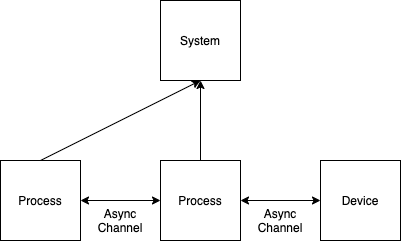
\includegraphics{../src/tex/system.png}

Processes within the same system can communicate with each other or
with devices. Processes in distinct systems must use a device as
a middleman to communicate.

\section{Processes}
The execution of a process is effected by one or more {\em threads}.
If there is only one, the process is {\em single threaded,} otherwise
if there are two or more, {\em multi-threaded.} Every process is started
with a single {\em initial} thread.

A {\em fibre} is a logical thread of control and associated execution
context. Each process consists of a collection of fibres. 

Fibres in a process are {\em running} if a thread is elaborating the
fibre's program code, otherwise the fibre is {\em suspended}. 

A suspended fibre can either be {\em ready} or {\em waiting}.
The collection of ready and running fibres are said to be {\em active}.

All the ready fibres of a processes are maintained in a set and
are owned by their process. Running fibres are owned by the thread
running them which are owned by the thread's process.

When a thread is out of work, it attempts to locate a 
ready fibre the and run it. If there are no ready fibres,
no fibres are running, and there are no fibres waiting on
asynchronous I/O from an external device or another system,
then the process terminates and all associated memory is released,
all but the initial thread are terminated, and the initial thread
returns control.

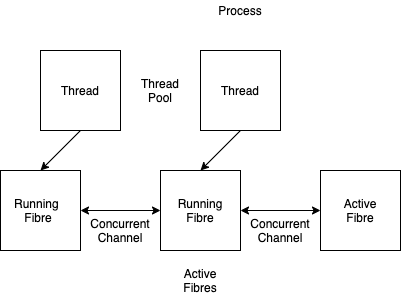
\includegraphics{../src/tex/process.png}


\section{Fibres}

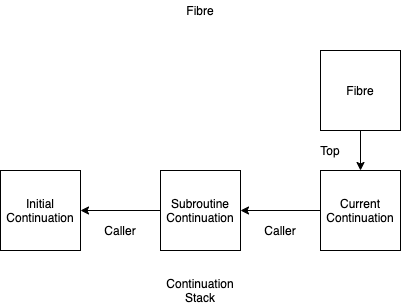
\includegraphics{../src/tex/fibre.png}


\end{document}
